\chapter{Equation of State, Radiation, and Vacuum Energy}

These companion notes follow Leonard Susskind's fifth lecture in the Cosmology course, with curation support by LazyingArt LLC and Video2Book. The lecture is organized around a simple but decisive question: if cosmology is, to first approximation, the history of the scale factor \(a(t)\), what input tells us how the right-hand side of the Friedmann equation changes as the universe expands? The answer is the equation of state. We will first recover the density-scaling law from a thermodynamic box argument, then derive \(w=\tfrac13\) for radiation from photon momentum flow, and finally turn to vacuum energy, for which \(w=-1\) and the cosmic evolution becomes qualitatively different.

\section{Review: The Scale Factor and Why the Equation of State Matters}

The lecture begins by stepping back. Before adding anything new, we are reminded what the main question of cosmology has been all along: what is the history of the universe? In the homogeneous and isotropic approximation, that question reduces to the time history of one quantity, the scale factor \(a(t)\). If we know \(a(t)\), we know an enormous amount about the large-scale story.

Two benchmark models have already appeared:
\begin{equation}
a(t)\propto t^{2/3}
\qquad\text{(matter domination)},
\end{equation}
and
\begin{equation}
a(t)\propto t^{1/2}
\qquad\text{(radiation domination)}.
\end{equation}
Neither law is exact for all times. Radiation is the right approximation earlier; matter is the right approximation later. But the important point in the review is not merely the pair of exponents. The real question is what distinguishes the two cases on the right-hand side of the cosmological equations.

\begin{figure}[h]
\centering

\includegraphics[width=0.72\textwidth]{lecture_05_figure_02.png}
\caption{Reviewed scale-factor laws with newly introduced energy-density notation.}
\end{figure}

This frame is a transition rather than a finished derivation, but it captures the essential turn in the lecture: from known scale-factor laws to the energy density \(\rho\). The equation of state, Susskind says, is precisely what tells us how that energy density changes when the universe expands. In the two cases already on the table, the corresponding density laws are
\begin{equation}
\rho_{\text{matter}}=\frac{\rho_0}{a^3},
\qquad
\rho_{\text{rad}}=\frac{\rho_0}{a^4}.
\end{equation}
The matter law is easy to recognize: matter simply dilutes with the volume, and volume scales like \(a^3\). Radiation is the more interesting case. Its density falls with one extra power of \(a\). The lecture now asks where that extra factor comes from, and more generally what relation between pressure and energy density produces these scaling laws.

\section{From \(P=w\rho\) to the Density-Scaling Law}

In cosmology we simplify the equation of state to the linear form
\begin{equation}
P=w\rho,
\end{equation}
where \(w\) is a number characterizing the fluid. The board writes an uppercase \(W\), but we will normalize to the conventional lowercase \(w\).

Before turning to the general derivation, Susskind briefly motivates the first case physically. For nonrelativistic matter, the energy density comes mainly from rest mass, hence from \(mc^2\). Pressure, on the other hand, comes from particles striking a wall, and that depends on their comparatively small velocities, not on the speed of light. Therefore the pressure is tiny compared with the energy density, so \(w\approx 0\). Radiation will be very different, but that difference will be proved rather than asserted.

What we now want is a general machine that turns an equation of state into a scaling law for \(\rho\). The lecture gets that machine from a thermodynamic box.

\begin{figure}[h]
\centering

\includegraphics[width=0.86\textwidth]{lecture_05_figure_03.png}
\caption{Equation of state and thermodynamic box argument.}
\end{figure}

This board state is especially useful because it preserves the lecture's whole layout. On the left sit the previously reviewed cosmological scalings. On the right the lecture starts over with the abstract equation of state and the box sketch. Read together, the board is saying:
\begin{equation}
\rho_{\text{matter}}=\frac{\rho_0}{a^3},
\qquad
\rho_{\text{rad}}=\frac{\rho_0}{a^4},
\qquad
P=w\rho.
\end{equation}
The point is to derive the left-hand formulas from the right-hand one.

We imagine a box of gas. One wall has area \(A\), and we move it outward by a small distance \(dx\). Then
\begin{equation}
dV=A\,dx.
\end{equation}
The force on the wall is \(PA\), so the work done by the gas during the displacement is \(PA\,dx=P\,dV\). Since the gas does the work, the energy left inside the box decreases:
\begin{equation}
dE=-P\,dV.
\end{equation}

\begin{figure}[h]
\centering
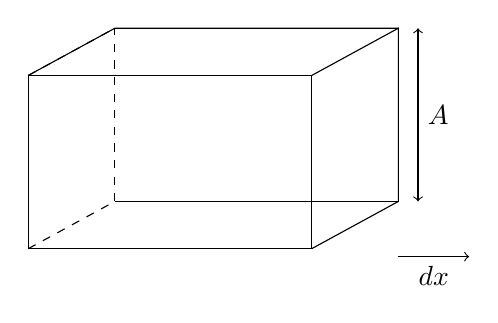
\begin{tikzpicture}[scale=1.0]
\draw (0,0) -- (3.6,0) -- (3.6,2.2) -- (0,2.2) -- cycle;
\draw (3.6,0) -- (4.7,0.6) -- (4.7,2.8) -- (3.6,2.2);
\draw (0,2.2) -- (1.1,2.8) -- (4.7,2.8);
\draw (1.1,0.6) -- (4.7,0.6);
\draw[dashed] (0,0) -- (1.1,0.6);
\draw[dashed] (0,2.2) -- (1.1,2.8);
\draw[dashed] (1.1,0.6) -- (1.1,2.8);
\draw[<->] (4.95,0.6) -- (4.95,2.8);
\node[right] at (4.95,1.7) {\(A\)};
\draw[->] (4.7,-0.1) -- (5.6,-0.1);
\node[below] at (5.15,-0.1) {\(dx\)};
\end{tikzpicture}
\caption{A clean redraw of the thermodynamic box used in the lecture.}
\end{figure}

Next comes the key substitution:
\begin{equation}
E=\rho V.
\end{equation}
Differentiating gives
\begin{equation}
d(\rho V)=\rho\,dV+V\,d\rho.
\end{equation}
Substituting this into the work relation,
\begin{equation}
\rho\,dV+V\,d\rho=-P\,dV.
\end{equation}
Now insert the equation of state \(P=w\rho\). Then
\begin{equation}
V\,d\rho=-(1+w)\rho\,dV.
\end{equation}
At this stage, as the lecture likes to say, the equation is becoming famous, but it is not famous yet. Divide by \(\rho V\):
\begin{equation}
\frac{d\rho}{\rho}=-(1+w)\frac{dV}{V}.
\end{equation}
This is the separated form shown clearly on the board.

\begin{figure}[h]
\centering

\includegraphics[width=0.78\textwidth]{lecture_05_figure_04.png}
\caption{Logarithmic integration of the density-volume relation.}
\end{figure}

The lecture frame shows the separated equation and the beginning of the logarithmic line, \(\log\rho=\). The full integrated form is a cautious standard completion of what is already on the board:
\begin{equation}
d(\log\rho)=-(1+w)\,d(\log V),
\end{equation}
so that
\begin{equation}
\log\rho=-(1+w)\log V+\text{const.}
\end{equation}
Exponentiating,
\begin{equation}
\rho\propto V^{-(1+w)}.
\end{equation}
Now the equation has become famous.

Finally we return from the box to cosmology. Under isotropic expansion the volume of a comoving region scales as
\begin{equation}
V\propto a^3.
\end{equation}
Therefore
\begin{equation}
\rho\propto a^{-3(1+w)}.
\end{equation}
That is the general density-scaling law the lecture has been heading toward.

\section{First Applications: Matter and Radiation}

Now we go back and check that the review formulas really do emerge from the general argument.

For nonrelativistic matter we take
\begin{equation}
w=0.
\end{equation}
Then
\begin{equation}
\rho\propto a^{-3},
\end{equation}
which is exactly the matter-dilution law we started with.

For radiation the lecture announces the answer and then promises to prove it:
\begin{equation}
w=\frac13.
\end{equation}
If this is correct, then
\begin{equation}
\rho\propto a^{-3(1+1/3)}=a^{-4}.
\end{equation}
So the opening review is now seen in its proper order. The lecture began with \(a(t)\sim t^{2/3}\) and \(a(t)\sim t^{1/2}\), then asked what input distinguishes them, and now the general scaling law has shown that the answer lies in the equation of state. Only one crucial step remains unresolved: why does radiation have \(w=\tfrac13\)?

\section{Why Radiation Has \(w=\frac13\)}

At this point the lecture narrows to a single task. Radiation means massless particles; for our purposes that means photons. The characteristic difference from nonrelativistic matter is not subtle: photons move with the speed of light. So if we want the radiation equation of state, we must compute the pressure produced by a gas of photons.

Susskind introduces notation carefully. Let \(\epsilon\) be the energy per photon, and let \(\vec{\pi}\) be the photon momentum vector. The usual symbol \(p\) is avoided because \(P\) is already reserved for pressure. For a massless particle,
\begin{equation}
\epsilon=c\,\pi,
\end{equation}
with \(\pi=|\vec{\pi}|\). In the units used in the lecture, \(c=1\), so
\begin{equation}
\epsilon=\pi.
\end{equation}
If \(\nu\) is the photon number density, then the energy density is
\begin{equation}
\rho=\epsilon\,\nu.
\end{equation}

Now we compute the pressure on a wall. Let the \(x\)-axis be normal to the wall. During a short time interval \(\Delta t\), a photon moving at angle \(\theta\) to the normal will hit the wall only if it starts inside a slab of thickness
\begin{equation}
\Delta x=\Delta t\cos\theta.
\end{equation}
If it reflects, its \(x\)-component of momentum reverses sign, so the momentum transferred to the wall is
\begin{equation}
\Delta \pi_x=2\epsilon\cos\theta.
\end{equation}
Force is momentum transfer per unit time, so one hit contributes \(\Delta \pi_x/\Delta t\). The number of photons in the slab is \(\nu A\Delta x\), but only half of them move toward the wall, so the relevant number is \(\tfrac12 \nu A\Delta x\). Dividing the total force by the wall area \(A\), we find
\begin{align}
P(\theta)
&=
\frac{1}{A}
\left(\frac{2\epsilon\cos\theta}{\Delta t}\right)
\left(\frac12 \nu A\Delta x\right) \\
&=
\epsilon\nu\cos\theta\frac{\Delta x}{\Delta t} \\
&=
\epsilon\nu\cos^2\theta \\
&=
\rho\cos^2\theta.
\end{align}
The answer still depends on angle, but that is only because we have computed the contribution from photons traveling in one direction.

\begin{figure}[h]
\centering
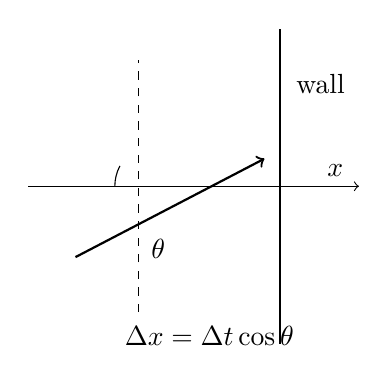
\begin{tikzpicture}[scale=1.0]
\draw[thick] (0,0) -- (0,4);
\draw[->] (-3.2,2) -- (1.0,2);
\node[above] at (0.7,2) {\(x\)};
\draw[dashed] (-1.8,0.4) -- (-1.8,3.6);
\node[below] at (-0.9,0.35) {\(\Delta x=\Delta t\cos\theta\)};
\draw[->,thick] (-2.6,1.1) -- (-0.2,2.35);
\node[below] at (-1.55,1.45) {\(\theta\)};
\draw (-2.1,2) arc[start angle=180,end angle=152,radius=0.55];
\node[right] at (0.08,3.3) {wall};
\end{tikzpicture}
\caption{Transcript-backed reconstruction of the photon-pressure geometry.}
\end{figure}

Now comes the conceptual hinge of the derivation. Let \(\mathbf n=(n_x,n_y,n_z)\) be the unit vector along the direction of motion of a photon. Then
\begin{equation}
n_x=\cos\theta,
\qquad
n_x^2+n_y^2+n_z^2=1.
\end{equation}
In an isotropic gas, the averages of \(n_x^2\), \(n_y^2\), and \(n_z^2\) are equal. Averaging the identity above,
\begin{equation}
\langle n_x^2\rangle+\langle n_y^2\rangle+\langle n_z^2\rangle=1,
\end{equation}
and by symmetry each term is the same, so
\begin{equation}
\langle n_x^2\rangle=\langle \cos^2\theta\rangle=\frac13.
\end{equation}
Therefore
\begin{equation}
P=\rho\langle \cos^2\theta\rangle=\frac{\rho}{3}.
\end{equation}
So the radiation equation of state is
\begin{equation}
P=\frac13\rho,
\qquad
w=\frac13.
\end{equation}
That closes the first major loop of the lecture: the review formulas for matter and radiation are now consequences of the equation of state rather than assumptions placed at the beginning.

\subsection{Question \& Answer}

\paragraph{Do we need all photons to have the same energy?} No. The equal-energy assumption is only a convenience. One can think of the calculation as being done separately for photons in each energy range; each range contributes pressure equal to one third of its own energy density, and summing over all energies leaves the same result.

\paragraph{What if the walls absorb rather than reflect?} The answer is still the same. In a black box at thermal equilibrium, absorbed photons are re-emitted, and the net momentum balance is unchanged. More importantly, in cosmology the box is only a local bookkeeping device. There are no literal walls in empty space. Photons cross an imagined surface, but on average the outward flux is balanced by an inward flux from the other side. The pressure is still momentum flow, and the same equation of state follows.

\paragraph{Do quantum statistics change the result?} Not here. The lecture is explicit that quantum statistics do not alter the conclusion \(P=\rho/3\).

\paragraph{What about photon-photon scattering?} In principle it can change the equation of state slightly, especially at very high temperatures where new channels such as electron-positron pair production open up. But under the conditions relevant to the lecture, the effect is negligible.

\paragraph{What happened to the area?} The lecture stops over this point on purpose. The intermediate quantity first computed is the total force. Pressure is only obtained after dividing by the wall area. The cancellation is therefore not an accident but exactly what must happen.

\section{Negative Pressure and the Meaning of Tension}

Up to now, pressure has been produced by particles bouncing around inside a box. That naturally suggests positive pressure: the contents push outward. The lecture now deliberately changes conceptual register and asks a new question. Can pressure be negative?

The answer is yes, and the lecture's bridge to that answer is tension. In a one-dimensional world, a box is just a line segment. If particles bounce between its ends, they push the walls outward and we get positive pressure. But suppose instead that the two ends of the interval are connected by a spring or a string. If we pull the walls apart, the spring pulls back inward. That inward pull is not pressure in the ordinary positive sense. It is tension, and tension is the one-dimensional model of negative pressure.

\begin{figure}[h]
\centering
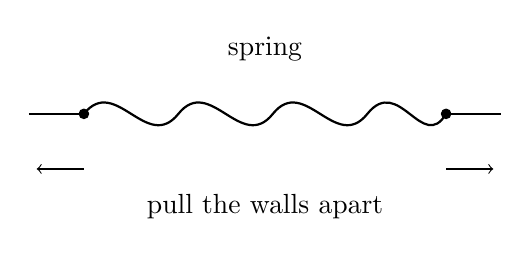
\begin{tikzpicture}[scale=1.0]
\draw[thick] (-3,0) -- (-2.3,0);
\draw[thick] (2.3,0) -- (3,0);
\draw[fill] (-2.3,0) circle (0.06);
\draw[fill] (2.3,0) circle (0.06);
\draw[thick] (-2.3,0)
.. controls (-1.9,0.5) and (-1.5,-0.5) .. (-1.1,0)
.. controls (-0.7,0.5) and (-0.3,-0.5) .. (0.1,0)
.. controls (0.5,0.5) and (0.9,-0.5) .. (1.3,0)
.. controls (1.7,0.5) and (2.0,-0.5) .. (2.3,0);
\draw[->] (-2.3,-0.7) -- (-2.9,-0.7);
\draw[->] (2.3,-0.7) -- (2.9,-0.7);
\node[below] at (0,-0.9) {pull the walls apart};
\node[above] at (0,0.55) {spring};
\end{tikzpicture}
\caption{A one-dimensional spring as an analogy for negative pressure.}
\end{figure}

This also changes the energy bookkeeping. For ordinary positive pressure, when the box expands the system does work and the energy inside decreases. For tension, when we pull outward against the spring, we store more energy in the configuration. So negative pressure is not just an odd sign choice in an equation. It is a recognizable physical behavior once we stop imagining only dilute particles striking the wall.

\subsection{Question \& Answer}

\paragraph{How can pressure be negative while the energy density stays positive?} The spring makes the answer concrete. The system may contain positive stored energy and nevertheless pull inward. In that case \(P<0\) while \(\rho>0\), so \(w=P/\rho\) is negative.

\paragraph{Why is this important in cosmology?} Because the lecture is about to introduce precisely such a medium. If negative pressure were a mere curiosity, it would not deserve this much attention. It matters because vacuum energy behaves in this way.

\section{Vacuum Energy, the Cosmological Constant, and \(w=-1\)}

We are now ready for the stranger fluid. Vacuum energy is the energy density of empty space itself. Whatever its microscopic origin may be, its defining macroscopic property is simple and radical: the energy density of the vacuum does not dilute when we enlarge the box. It is a property of space, not a quantity of stuff being spread thinner.

So we write
\begin{equation}
\rho=\rho_0=\text{const.}
\end{equation}
If a region of volume \(V\) contains only vacuum energy, then the total energy in that region is
\begin{equation}
E=\rho_0 V.
\end{equation}
At this stage the lecture introduces a second symbol,
\begin{equation}
\Lambda=\frac{8\pi G}{3}\rho_0.
\end{equation}
This is just a definition, but it is the useful definition, because the combination \(8\pi G\rho/3\) is what appears naturally in the Friedmann equation. In the language of the lecture, \(\Lambda\) appears more nicely in cosmology than \(\rho_0\) itself. It is the cosmological constant, and in more recent language it is also what newspapers call dark energy.

The scale-factor dependence is already settled: there is none. Vacuum energy does not change when the universe expands. But the lecture then asks a further question for fun and for physics: what equation of state corresponds to that behavior?

We answer by running the box derivation backward. Since \(\rho_0\) is constant,
\begin{equation}
dE=d(\rho_0V)=\rho_0\,dV.
\end{equation}
On the other hand the thermodynamic work relation is still
\begin{equation}
dE=-P\,dV.
\end{equation}
If we write \(P=w\rho_0\), then
\begin{equation}
dE=-w\rho_0\,dV.
\end{equation}
Comparing these two expressions for \(dE\), we obtain
\begin{equation}
w=-1.
\end{equation}
So the equation of state of vacuum energy is
\begin{equation}
P=-\rho.
\end{equation}
This is the exact point the spring analogy was preparing us for. If the vacuum energy density is positive, the pressure is negative. If the vacuum energy density is negative, the pressure is positive. That is the characteristic signature of vacuum energy.

\subsection{Question \& Answer}

\paragraph{Does putting vacuum energy in a box change the density by restricting the allowed modes?} The lecture pauses over this point because it is a natural objection. The answer given there is no, not for the purposes at hand. Restricting the box changes the total energy because the volume changes, but the vacuum energy density itself is taken to be universal. The familiar Casimir effect is real, but it matters only when the walls are extremely close together. It is not the phenomenon being described here.

\paragraph{What do astronomers mean when they say they are measuring \(w\)?} They are testing whether the dominant late-time energy density behaves like vacuum energy. The closer the observed \(w\) is to \(-1\), the closer the cosmic fluid is to a genuinely nondiluting vacuum energy.

\section{Pure-Vacuum Cosmologies}

With the equation of state in hand, the lecture turns to dynamics. What does a universe do if the only energy density present is vacuum energy? In Susskind's normalization the Friedmann equation is
\begin{equation}
\left(\frac{\dot a}{a}\right)^2=\Lambda-\frac{k}{a^2},
\end{equation}
with \(k=+1,0,-1\) for spherical, flat, and hyperbolic spatial geometry.

\subsection{The flat case: de Sitter expansion}

The simplest case is \(k=0\). Then
\begin{equation}
\left(\frac{\dot a}{a}\right)^2=\Lambda.
\end{equation}
For positive \(\Lambda\), taking the positive square root gives
\begin{equation}
\dot a=\sqrt{\Lambda}\,a,
\end{equation}
and therefore
\begin{equation}
a(t)=C\,e^{\sqrt{\Lambda}\,t}.
\end{equation}
The Hubble parameter is then constant:
\begin{equation}
H=\frac{\dot a}{a}=\sqrt{\Lambda}.
\end{equation}
This is de Sitter space in flat slicing.

The lecture briefly notes, and then postpones, a subtlety: this slicing is not geodesically complete, so the question of whether one should literally regard it as having a Big Bang is more delicate than the exponential formula alone suggests. He does not pursue that issue here.

What he does emphasize is the transition from mixed cosmology to vacuum domination. If matter or radiation are also present, then schematically
\begin{equation}
\left(\frac{\dot a}{a}\right)^2
=
\Lambda+\frac{C_m}{a^3}+\frac{C_r}{a^4}-\frac{k}{a^2}.
\end{equation}
At early times, when \(a\) is small, the inverse powers dominate and vacuum energy is negligible. At late times, when \(a\) is large, the constant term \(\Lambda\) dominates. So the universe makes a transition: early on it looks matter- or radiation-dominated, while late on it approaches de Sitter-like behavior.

This is why the lecture says we are not yet seeing a pure exponential era, but are beginning to see a departure in that direction. The expansion is accelerating. If \(a(t)\) were exactly exponential, then both \(\dot a\) and \(\ddot a\) would also be exponential; the universe would not only expand, it would expand at an accelerating rate.

\subsection{Question \& Answer}

\paragraph{Why is dark energy mysterious?} The lecture insists on a specific answer. What is mysterious is not that vacuum energy exists, but that there is so little of it. A bosonic mode contributes \(+\tfrac12\hbar\omega\) to the vacuum energy, and a fermionic mode contributes \(-\tfrac12\hbar\omega\). Exact supersymmetry would make these contributions cancel exactly, but nature does not exhibit that exact matching. So the shock is not the presence of vacuum energy, but its enormous smallness.

\paragraph{How small?} As presented in the lecture, the observed vacuum energy density is about \(123\) orders of magnitude below the naive Planck-scale estimate. The lecture treats this as a perspective statement rather than as a derivation, but it is the right perspective statement.

\paragraph{Does \(w=-1\) have to be exact?} In the lecture the observational situation is described as consistent with \(w=-1\) to within roughly ten percent, with the expectation that observations may narrow that window further. The conceptual point is the same: measuring \(w\) is measuring how vacuum-like the dominant energy density really is.

\subsection{Positive curvature with positive \(\Lambda\)}

The lecture now turns to a less trivial case: \(k=+1\) with \(\Lambda>0\). Then
\begin{equation}
\left(\frac{\dot a}{a}\right)^2=\Lambda-\frac{1}{a^2}.
\end{equation}
Multiplying by \(a^2\),
\begin{equation}
\dot a^2-\Lambda a^2=-1.
\end{equation}
Here Susskind changes idiom and translates the Friedmann equation into mechanics. If \(a\) is viewed as the coordinate of a fictitious particle, then \(\dot a^2\) plays the role of kinetic energy and \(-\Lambda a^2\) the role of an upside-down quadratic potential. The total energy is fixed at \(-1\). The motion is therefore bounce-like: the particle climbs, stops, and falls back.

The exact solution quoted in the lecture is
\begin{equation}
a(t)=\Lambda^{-1/2}\cosh(\sqrt{\Lambda}\,t).
\end{equation}
Using
\begin{equation}
\cosh(\sqrt{\Lambda}\,t)
=
\frac12\left(e^{\sqrt{\Lambda}\,t}+e^{-\sqrt{\Lambda}\,t}\right),
\end{equation}
we see that the solution is symmetric in time. At late positive times it looks exponentially expanding, just as in the flat case. But globally it describes a universe that contracts, reaches a minimum size, and then re-expands. In this slicing the geometry is naturally described as a bounce.

\subsection{Negative cosmological constant}

Suppose now that \(\Lambda<0\). If \(k=+1\), then the right-hand side of the Friedmann equation is negative while the left-hand side is nonnegative, so there is no solution.

The interesting case is \(k=-1\) with negative cosmological constant. Setting \(|\Lambda|=1\) to reduce clutter, we have
\begin{equation}
\left(\frac{\dot a}{a}\right)^2=-1+\frac{1}{a^2}.
\end{equation}
Multiplying through by \(a^2\),
\begin{equation}
\dot a^2+a^2=1.
\end{equation}
Now the mechanical analogy is a harmonic oscillator. The potential is an ordinary upward quadratic well and the total energy is fixed. Since \(a\geq 0\), only half of the oscillation is physically relevant: the universe expands from \(a=0\), reaches a maximum size, and collapses again. So even an open universe can end in a big crunch if the cosmological constant is sufficiently negative.

\begin{figure}[h]
\centering
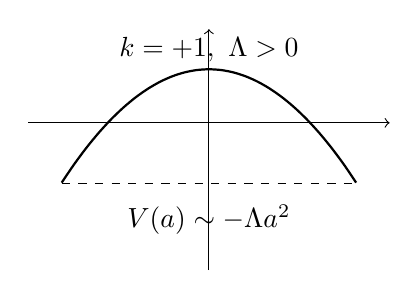
\begin{tikzpicture}[scale=0.85]
\draw[->] (-2.7,0) -- (2.7,0);
\draw[->] (0,-2.2) -- (0,1.4);
\draw[thick,domain=-2.2:2.2,smooth] plot (\x,{-0.35*(\x)^2 + 0.8});
\draw[dashed] (-2.2,-0.9) -- (2.2,-0.9);
\node at (0,-1.45) {\(V(a)\sim -\Lambda a^2\)};
\node at (0,1.1) {\(k=+1,\ \Lambda>0\)};
\end{tikzpicture}
\hspace{2em}
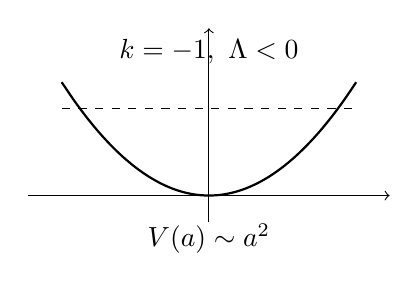
\begin{tikzpicture}[scale=0.85]
\draw[->] (-2.7,0) -- (2.7,0);
\draw[->] (0,-0.4) -- (0,2.5);
\draw[thick,domain=-2.2:2.2,smooth] plot (\x,{0.35*(\x)^2});
\draw[dashed] (-2.2,1.3) -- (2.2,1.3);
\node at (0,-0.65) {\(V(a)\sim a^2\)};
\node at (0,2.15) {\(k=-1,\ \Lambda<0\)};
\end{tikzpicture}
\caption{Transcript-backed schematic potentials for the mechanical analogies used in the lecture.}
\end{figure}

One final caution from the end of the lecture should not be dropped. The ansatz \(P=w\rho\) is useful and covers the important cases discussed here, but it is not a theorem about all fluids. A general fluid need not satisfy a linear relation of this sort, and mixtures of fluids certainly do not behave as a single constant-\(w\) medium across all epochs.

\section{Summary}

The lecture opens by recentering cosmology on its main problem: the time history of the scale factor \(a(t)\). The equation of state is then introduced as the missing input that tells us how the energy density on the right-hand side of the Friedmann equation changes during expansion. From the thermodynamic box argument we obtain the general law
\[
\rho\propto a^{-3(1+w)}.
\]
Matter gives \(w=0\) and so \(\rho\propto a^{-3}\). Radiation gives \(w=\tfrac13\) and so \(\rho\propto a^{-4}\). The radiation result is not postulated; it is derived from photon momentum transfer and the isotropic average \(\langle\cos^2\theta\rangle=\tfrac13\).

The lecture then turns to negative pressure. Tension provides the physical bridge, vacuum energy the cosmological example, and the backward box argument gives \(w=-1\). With that in hand, the pure-vacuum Friedmann equation yields flat de Sitter expansion for \(k=0\), a bounce-like \(\cosh\) solution for \(k=+1\) and positive \(\Lambda\), and re-collapse for \(k=-1\) with negative \(\Lambda\). The chapter closes where the lecture closes: vacuum energy is not mysterious because it exists, but because it is almost absent.